\chapter{Technical background}
\label{chapter:technical background} 

In the following section we focus on the Column-oriented datastores, explained before, and in particular in the HBase solution, one of the most popular and open-source Column-oriented datastores.

\section{Column-Oriented Datastores}

When referring to Column-Oriented datastores, also called Extensible Record Stores, where BigTable is the pioneer. BigTable and many other datastores of this type present a simple and flexible data model that can be extended at any moment.
Some famous Column-Oriented datastores are Apache HBase \cite{ApacheHBase}, HyperTable \cite{HyperTable}, Apache Accumulo \cite{ApacheAccumulo}, and Apache Cassandra \cite{ApacheCassandra} in addition to many others.
\par
Among all these solutions, HBase \cite{george2011hbase} is likely the most popular open-source Column-Oriented datastore and is the one that we are going to use for our experiments.
\par
In the next section, we will describe HBase and how it works in order to fully understand this Thesis.


\section{HBase}


HBase is an important Apache Hadoop-based project, which, as we stated before, is modeled on Google's BigTable database. HBase can be characterized as a distributed, fault tolerant scalable database built on top of the HDFS file system. It belongs to the group of column-oriented datastores and uses  Apache ZooKeeper for management of partial failures.
\par
Below, all must-known aspects of HBase are presented: HBase data model, storage, architecture, write/read/delete paths and the client API.


\subsection{Data Model}

HBase stores data items, those are key/value pairs. The keys are multidimensional. Each single value is indexed by a row key, column key and a timestamp \footnote{Timestamp, also known as version number}. Row keys are unique and allow the user to address all columns in one logical row. The column key is the combination of a column family and a column qualifier. Column families are the main unit of separation within a table. The last part is the timestamp which is used for versioning the data. Timestamp is usually automatically generated by the corresponding Region Server but it can be specified by the user.
\par
Summarizing, a key is commonly represented as the tuple (row, column, timestamp), which addresses a specified value:

\bigskip

			\centerline{\textbf{(row, column, timestamp) -\textgreater value}}

\bigskip 
\par
where column equals (column family, column qualifier), timestamp is a 64-bit integer and row, column family, column qualifier and value are uninterpreted array strings, since in HBase everything is store as bytes.

\begin{table}[htbp]
\begin{center}
\begin{tabular}{|l|l|l|l|}
\hline
\textbf{Row Key} & \textbf{Time Stamp} & \textbf{Family:Qualifier} & \textbf{Family:Qualifier} \\ \hline
"com.cnn" & t9 &   & anchor:cnnsi = "Y" \\ \hline
"com.cnn" & t8 &   & anchor:look = "X" \\ \hline
"com.cnn" & t6 & contents:html = "" &   \\ \cline{1-2}
"com.cnn" & t5 & contents:html = "" &   \\ \cline{1-2}
"com.cnn" & t3 & contents:html = "" &   \\ \hline
\end{tabular}
\caption{Example HBase table given by \cite{ApacheHBaseDataModel}}
\end{center}
\end{table}

A cell is a set of data items with a common row and column key (remember that column key stands for (column family:column qualifier)), being the cell key = (row, column). Each data item in a cell is called a version of that cell.
\par
HBase supports multiple versions of cells. Each version of a cell is stored as a separated cell, next to other versions of that cell. Versions of a cell are sorted descending by the timestamp so that users will see the newest value first while reading it.
Another HBase table feature is that it does not store NULL values as RDBMSs do. Files storing the data only contain data explicitly set.
\par
A table is organized by grouping cells into rows. These cells are sorted lexicographically by row key first and then by column key, so row keys lexicographically close will be stored near to each other. The sorting allows the table to be partitioned into the denominated \textit{regions}, which hold exclusive ranges of row keys. The regions of a table are distributed between different nodes.

\subsection {Storage}

The real view of tables differs from the conceptual view explained before. Physically, tables are stored on a per-column family basis, which means that all column family members are stored together in files called HFiles/StoreFiles. Such an approach brings advantages, one of which is that they can be compressed together. Column families must be declared while creating the table, whereas column qualifiers can be added to column families at any time.
\par
As written before, the HBase storage files are called HFiles. They are based on Hadoop's TFile\footnote{{TF}ile {S}pecification - \url{https://issues.apache.org/jira/secure/attachment/12396286/TFile+Specification+20081217.pdf}} class and mimic the SSTable format used in Google's BigTable system. What is stored inside them is called KeyValue instances. They are the physical view of the conceptual cells. The whole cell, with its structured data (row length, key type, etc.) is what is a KeyValue object. Figure 3.1 shows a conceptual depiction of the KeyValue format.
\par

\begin{figure}[htb]
\centering
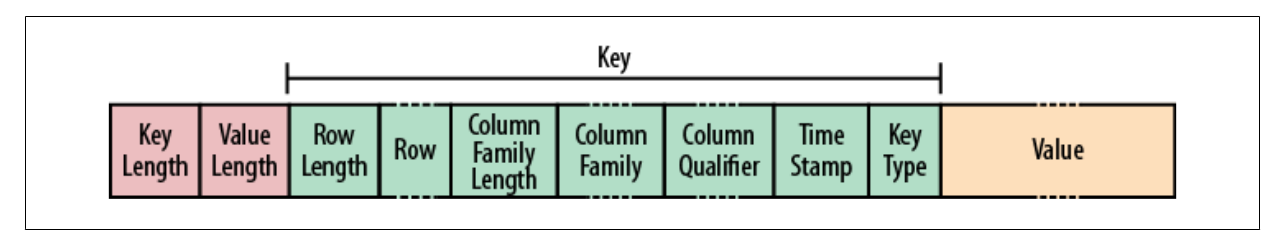
\includegraphics[width=0.8\textwidth]{./images/keyvalue.png}
\caption{The KeyValue format, extracted from HBase: The definitive guide \cite{george2011hbase}.} \label{fig:keyvalue}
\end{figure}


\subsection{Architecture}

HBase consists of three layers: the client, the server and the storage layers. The server layer consists of a master server and many region servers; the client has the library to communicate with the existing HBase installation; the storage layer is composed of a file system and a coordination service. Hadoop Distributed File System (HDFS) is the most used and tested file system to work with HBase. As the coordination service, ZooKeeper is the one HBase uses for its distributed coordination service. In the following section each component is explained as well as some HBase's features.

\begin{figure}[htb]
\centering
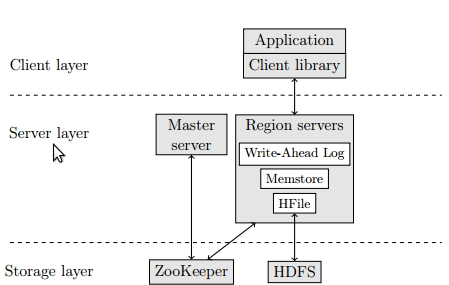
\includegraphics[width=0.8\textwidth]{./images/HBaseLayers.jpg}
\caption{HBase architecture overview} \label{fig:hbaselayers}
\end{figure}


\subsubsection{Storage layer}

The storage layer is composed of a chosen file system for the HBase cluster and a coordination service:

\begin{itemize}
\item File system: HDFS \cite{ApacheHadoop, HDFSarchitecture} is the default file system when deploying an HBase cluster, but optionally it can be replaced by any other file system. For HBase, HDFS is the primary option as it is scalable, fail safe, has automatic replication and is built to run on commodity hardware. It fits with the needs of a distributed system. 

% Hadoop MapReduce is always used with HDFS as the underlying file system, thereby HDFS performance when dealing % with a huge amount of data, as Hadoop MapReduce does, is optimized. 

\item Coordination service: Apache ZooKeeper \cite{ApacheZooKeeper, hunt2010zookeeper, junqueira2011zab} is an open source project and a part of the Apache Software Foundation. ZooKeeper is a highly-reliable distributed coordination service, comparable to Chubby \cite{burrows2006chubby}, owned by Google and used for BigTable. Its aim is to offer a file-system-like access to clients with directories and files (znodes) that are used to store data, register services or watch for updates in a simple interface. In HBase, every region server creates a node in ZooKeeper, which will be used by the master to discover them. HBase uses ZooKeeper to choose the unique master and to store "-ROOT-"'s address too.
Master server and region servers communicate with ZooKeeper to keep track of the current situation of the regions and region servers.
\end{itemize}
\subsubsection{Server layer}
Server layer is compound of two parts:
\begin{itemize}
\item Master: The master server does not store any actual data and is not part of the retrieval path. It is responsible for assigning regions to region servers, handling load balancing of regions across region servers, unloading busy servers and moving regions to servers that are freer, and performing garbage collection of files. Since it never stores or provides data to clients or region servers, is usually slightly loaded. Furthermore, it takes care of all administrative operations such as schema changes or creation of tables or column families.
\par
If the master server goes down, the cluster can still work as the HBase client does not talk with it directly. Nevertheless, master should be restarted as soon as possible.
\item Region: As Lars George states in his book HBase: The definitive guide \cite{george2011hbase}, a \textit{region} is the basic unit of scalability and load balancing in HBase and is responsible for storing the actual data. Inside it, we can see contiguous ranges of rows stored together. Clients communicate directly with region servers to run all retrieve / write data operations. Each region is served by only one region server, although each region server can store multiple regions. The region servers also split regions into two pieces at the row key which is in the middle of the whole region once they have exceeded the maximum allowed region size.
\end{itemize}

\subsubsection{Client layer}

Client needs to be able to find the region server which has a specific key. In order to achieve that, client communicates with the Zookeeper server and then retrieves the location of a table called "-ROOT-" table from there. This table stores information about all regions in the ".META." table, which is another table storing where regions are and its row key ranges. So client reads the ".META." table and receives the exact address of the correct region handling a determined key or key range. Thanks to this three level lookup, the client is able to find the correct region server and perform its operations. For optimizing the process, client caches region locations because once the user table region is known, it can be accessed straightforwardly without the three level lookup. Only if the region server informs the client that it is no longer serving a region, does the client a new three level lookup.


\subsection {Write}
This subsection clarifies how writes and related stuff are done in a such a complex system as HBase is.
\par
Write requests are served by Region Servers. These components have three main elements: Write-Ahead Log (WAL), Memstore and HFiles. The WAL acts as a log for all modifications done to data in that exact region, guaranteeing atomicity and durability. The WAL allows regions to recover from server failures. It contains all previous modifications and can be used to recover from and to replay the data, achieving the last known stable stage. Memstore is an in-memory buffer that contains recently updated data items sorted by key. It works similar to how write buffers work on microprocessors, MemStore buffers writings, thus reducing write latencies. There is one MemStore for each column family of a table in the region. HFiles stores actual HBase's data.
\par
HBase stores data to disk in a way similar to how a Log-Structured Merge Tree works \cite{o1996log}. First, when new data arrives at the region server it is put on the Write-Ahead Log (WAL). If the write to the WAL is achieved, the region server writes the data into the memory store. Region continues writing data to the Memstore until a configured maximum size. Once that threshold is reached, Memstore flushes the data to disk. When flushing, multiple HFiles are created, one per column family, which can affect negatively to HBase performance. Massive amounts of tiny files stand for more seeks and thus, higher latencies while reading. Due to that fact, HBase monitors the number and size of these files and does compactions from time to time. A compaction is the process of merging multiple HFiles together,  and there are two types:
\begin{itemize}
\item Minor compaction: It is responsible for rewriting the last few files into a larger one. It is triggered when certain properties and ratios are reached.
\item Major compaction: It merges all files of a region into one single file. It is usually triggered every twenty-four hours or even more due to heavy load. Sometimes, it is recommended to disable major compactions and manage them manually as they incur a high performance penalty due to rewriting all of the database contents.
\end{itemize}

HFile files store an index at the end of the file to locate blocks within the HFile. The index is loaded into memory when the HFile is opened allowing look-ups to be performed with a single disk seek. For a more complete overview of how these files are designed refer to \cite{white2012hadoop}.

\subsection{Read}
This paragraph explains reads in HBase. First of all, when a Region Server receives a Get request, it checks whether the desired row is in the MemStore or not. If not, it starts to search through the HFiles starting from the newest working towards older HFiles, which means to take a look through the disk contents because the data could be spread over multiple files.

\subsection{Delete}
Here we explain how data is deleted from a HBase cluster. We must be clear that rows are never directly erased from HBase. When a Region Server receives a Delete request, it looks for the row and writes a delete marker to it. Whenever a Get request tries to access a row that has been previously deleted, it will find the delete marker and data will not be returned. During the next major compaction, rows with the delete marker will finally be deleted.

\subsection {HBase API}

HBase provides a powerful client API written in Java as HBase does. It provides from basic operations to expensive ones. The initial set of basic operations are called CRUD operations which stands for "Create, Read, Update and Delete".

\bigskip


\textbf{Put Operation} 

There are two groups of Put operations, first one works on single rows and the other works on a list of rows, both allow users to store data into HBase's tables in a transparently manner. Defined as:
\par
\bigskip
\centerline{\textit{put([List]Put put[s])}}
\bigskip

The user needs to supply a Put object or a list of them. These Put objects are created with the Put constructor:
\par
\bigskip
\centerline{\textit{Put(byte[] row)}}
\bigskip
A row key is supplied in order to create the Put instance, and once the user has created it, he/she can start to add values to the specified Put instance with the \textit{Put.add(value)} method. The user can also supply a version number for a given key/value pair (timestamp), but if it is not specified, HBase gives to it a version number created from the current time of the Region Server responsible for that given row.
\par
When providing the value for the \textit{Put.add()} method, as opposed to what happens with column qualifiers that can be whatever the user needs, an existing column family need to be given. Column families are usually defined when creating tables, but the user can always add new families calling to an expensive operation. It is because of that, HBase heavily recommends users to use fixed column families, although they can be altered.
Unlike column families, new column qualifiers, version numbers and row keys can be provided on-the-fly within Put operations with no extra cost.
\par
The HBase API allows to use a built-in client-side write buffer that collects sets of Put operations before sending them as a unique RPC connection to the corresponding server. Hence, less RPC connections are needed resulting in an increase of the overall performance. HBase is smart enough to group and sort Puts by Region Server. If write buffer is not used,  any time a Put operation is completed, HBase's API will submit it to the right Region Server.

\bigskip
\textbf{Atomic Compare-and-Set Operation}

As a variation to the Put calls, the user can use Check and Put operation, defined as:
\par
\bigskip
\centerline{\textit{checkAndPut(byte[] row, byte[] family, byte[] qualifier,byte[] value, Put put)}}
\bigskip
This method allows users to issue Puts with a checking point. Only if the check step is successfully completed, the put operation is performed, everything as an atomic operation. It is really useful when dealing with data that needs previous values or similar stuff.
\par
All rows inside the Put object must be equal to the given row. The user can not use this operation to check different row keys. Otherwise, Check and Put operation will fail.

\bigskip
\textbf{Get Operation}

Like in HBase Put method, there are two groups of Get operations, the ones that work on a single row and the others that operate with multiple rows. Both allows the user to retrieve data stored in HBase's tables.
\par
Get operation is defined as:
\par
\bigskip
\centerline{\textit{get([List]Get get[s])}}
\bigskip
The user needs to supply a Get object. These objects are created with the Get constructor like in Put operations. it is:
\par
\bigskip
\centerline{\textit{Get(byte[] row)}}
\bigskip
In analogy with Put constructor, the user provides a row key to the Get method in order to get a Get instance. Get operation is bounded to a specified row, but can retrieve any data stored in it, from one value to all columns with its values.
\par
The user can add parameters to the Get object in order to narrow down the search. They will act as filters. If the user wants everything of a row, no filters are used, but if the user only wants a column family, the \textit{Get.addFamily()} method must be used. Same thing happens if the user only wants a column qualifier from a column family (\textit{Get.addColumn()}), or the row with a known timestamp (\textit{Get.setTimeStamp()}).
Lastly, there are methods, acting as filters, that allow users to specify how many versions want to be retrieved (\textit{Get.setMaxVersions()}) and many others.
\par
Like in Put method, the user can retrieve a list of Gets, instead of only one row. The main difference is that the user issues a list of Gets, instead of one Get object. The result will be an array of Results, one for each Get instance.

\bigskip
\textbf{Delete Operation}

HBase client API provides a method to delete data from its tables. Delete method is defined as:

\par
\bigskip
\centerline{\textit{delete([List]Delete delete[s])}}
\bigskip
Once more, the user is able to delete one row by one row or a list of them, the difference is the type of parameter: a Delete instance or a list of them.
\par
As with Get and Put calls, the user has to create a Delete instance and then adds details (filters) about the data he/she wants to remove, the constructor is:

\par
\bigskip
\centerline{\textit{Delete(byte[] row)}}
\bigskip

A row is provided. Subsequently, what user wants to be removed is added to it using different methods. Most important ones are \textit{Delete.deleteFamily()} method, used to remove an entire column family, including all its columns, and \textit{Delete.deleteColumns()} method, which operates on one column of a given column family, deleting all versions contained or just the cells matching the timestamp if it is provided. There are other types of Delete methods, but less used.

\bigskip
\textbf{Atomic Compare-and-delete Operation}

As a variation to the Delete call, the user can use Check and Delete operation. It is defined as:

\par
\bigskip
\centerline{\textit{checkAndDelete(byte[] row, byte[] family, byte[] qualifier, byte[] value, Del del)}}
\bigskip

It works as a Delete operation but adding a previous step in which a specify row key, column family, column qualifier and value are checked before deleting the desired row.
\par
Users can only check and delete on the same row. If the row key differs from the one pointed by the Delete instance, the CheckandDelete operation will fail.

\par
\textbf{Useful hint. }Row Locks for Row mutations:

Previous operations: Put, Delete and CheckAndDelete are executed in such a way that they guarantee row level atomicity. They are executed entirely. A row lock is provided by the corresponding Region Server, protecting the row from other users trying to access it. Not from users trying to read it, only for those submitting row mutations operations.

\bigskip
\textbf{Scan Operation}

Scan operation allows the user to scan a range of data, from one row to a determinate stop row, taking advantage of the underlying sequential storage layout HBase has. The scan returns every row between the chosen range of rows. This operation is not executed atomically, it can be partially executed. Hence, returned data can be outdated if there has been a write operation during the scan. 
\par
Scan operation is really similar to Get method and it works as a iterator, it means that user has a Scan instance and he/she must iterate over it to get all the results.
\par
Scan method is defined as:
\par
\bigskip
\centerline{\textit{getScanner(Scan scan)}}
\centerline{\textit{getScanner(byte[] family)}}
\centerline{\textit{getScanner(byte[] family, byte[] qualifier)}}
\bigskip
Each of them narrow the read data, from a general Scan to one that only returns values from a Column Family and inside it, from a Column Qualifier.
\par
As in Put or Get methods, Scan object is created with its constructor, which is:
\par
\bigskip
\centerline{\textit{Scan(byte[] startRow, byte[] stopRow)}}
\bigskip

It returns a Scan instance. Start row is mandatory and always inclusive, while stop row is not and is exclusive ( [startRow, stopRow) ). The user can submit filters as well.
\par
Once the user has created the Scan instance, the user can narrow the scanned data using \textit{Scan.addFamily()} method or even a more restricted  one which is, \textit{Scan.addColumn()}. There are more mechanisms that allows users to set timestamps or time ranges.
\par
It is important to notice that the Scan operation do not cover all results within a single RPC connection, but instead it returns row by row since they can be very large. In order to iterate over the results, Scan presents \textit{next()} and \textit{next(int nbRows)} methods. Using them, each call will be traduce to a RPC for every row.
\par
Summarizing, HBase Scan method can be seen as  a lot of Gets operations, and indeed, it is what it does.


\subsection{HBase properties}

In this section we discuss the CAP theorem and the BASE and the ACID model for HBase. 
\par
HBase is called a CP type system since it supports Consistency and Partition Tolerance facets of the CAP model.
HBase offers Partition Tolerance as it survives message loss due to server failures, network problems, etc. If a region server collapses, other nodes take over the tasks which comprised the region by replaying its commit log and memStores.
Regarding consistency, HBase does trade some availability to achieve a stronger level of consistency. After a write completes, the next read will see the lastest value because at any given time only one region server is responsible for that key.
Availability is given up because if a region server dies, its data will be unavailable until another region server comes up and picks up the died regions.
\par
HBase is not an ACID compliant database, but it guarantees some ACID properties, such as atomicity within a single row but not across multiple rows, or strong consistency thanks to the design of regions only being hosted in one region server at any one time, which creates only one responsible for serving a given data and also thanks to the Multi-Version Concurrency Control (MVCC) \footnote{MVCC \cite{bernstein1983multiversion} is a solution that keeps a list of versions of each data item. From the point of view of the user, he or she will only see one data item, but from the system side, each update of the data item will correspond to a newer version number of the same data item. Thus there will be multiple versions stored, but only one is the latest.} used by HBase to manage concurrent access to the database (no locks are used as in old ACID SQL databases, instead timestamps \footnote{Timestamps, also called version numbers, are the MVCC data structures} offers all HBase needs to get all of ACID). HAcid is a project developed by A. Medeiros which implements a system transaction for HBase. HAcid gets an ACID compliant HBase database version. In order to understand how ACID can be implemented in HBase refer to HAcid \cite{HAcid} .



\section{HDFS}
%un poco de introduccion aqui
HDFS is the distributed file system of the Apache Hadoop open-source framework that provides high-throughput access to the stored data. It is scalable, fail safe, offers automatic replication and is built to run on a set of commodity hardware.
\par
HDFS consists of a master node called NameNode, and slave nodes called DataNodes. HDFS splits the data into equal size blocks and spread them across all available DataNodes in the cluster. Each block is replicated three times by default with at least one replica within the same node. The NameNode retains all metadata about blocks and replicas.

\begin{figure}[htb]
\centering
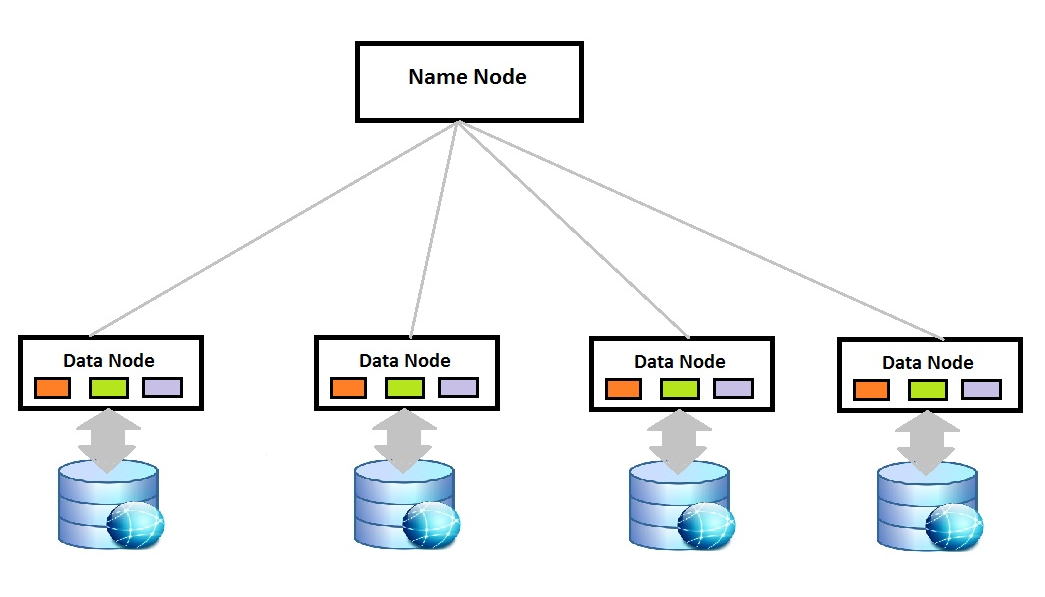
\includegraphics[width=0.8\textwidth]{./images/hdfs.png}
\caption{HDFS overview} \label{fig:hdfs}
\end{figure}


\section{MapReduce}

MapReduce programming model allows to abstract from the complexity of writing concurrent programs. It is based on two functions: map() and reduce(). The framework takes care of invoking them in the correct order on the input data and scheduling parallel execution of these two functions across any number of computation nodes. The user just needs to write the map and the reduce functions.
\par
Map takes an input as key/value pair (\textless k1, v1\textgreater), and emits a number of intermediate key/value pairs as its output (\textless k2, v2\textgreater). The MapReduce job group together all the values which have the same intermediate key and passes them to the Reduce function (\textless k2, list(v2)\textgreater).
\par
Reduce accepts intermediate key and a set of values for that key as input(\textless k2, list(v2)\textgreater). For each pair the reduce function outputs a final key/value pair (\textless k2, v3\textgreater). Map and reduce functions can be summarized in the following equations:

\centerline{map(\textless k1, v1\textgreater) \:\:  -\textgreater \:\:   list(\textless k2, v2\textgreater)}
\par
\centerline{reduce(\textless k2, list(v2)\textgreater) \:\:  -\textgreater \:\:  \textless k2, v3\textgreater}

\bigskip
\par

The MapReduce model fits with many large-scale data problems and can be efficiently implemented to support problems which input data is hundreds or thousands of megabytes. Due to the large size of the data, is more efficient and easier to move the computation instead the data. Therefore, in a MapReduce framework, data is split into blocks and distributed across many nodes in a cluster. Then, it is the MapReduce framework who takes advantage of data locality by moving computation to data rather than sending data to the nodes. That is, MapReduce schedules Map tasks close to the data block on which they will work, so it can be read and processed very fast for each node in parallel. This is the principal factor in MapReduce's performance.

\subsection{Hadoop MapReduce}

% for a more non-technical view, go to the introduction 1.

Hadoop MapReduce \cite{ApacheHadoop} \cite{white2012hadoop} is the popular Apache open-source Java implementation of the MapReduce model. It is always used with HDFS as the underlying file system. Hadoop MapReduce consists of a single master node called JobTracker and worker nodes called TaskTrackers. When using HDFS with Hadoop MapReduce, TaskTrackers live on the same nodes where HDFS DataNodes live.
\par
When a Hadoop MapReduce is submitted, it is divided into map tasks, also known as mappers, and reduce tasks, also called reducers. Each task is executed on a available slot in a worker node. Each worker can handle a fixed number of either mappers or reducers.
\par
The number of mappers is determined by the number of data blocks as each map task processes a block of input data. Each data block should be as close to the map task as possible, so data locality can be exploited and the amount of IO reduced. On the other hand, the number of reduce tasks is specified by the application.

\begin{figure}[htb]
\centering
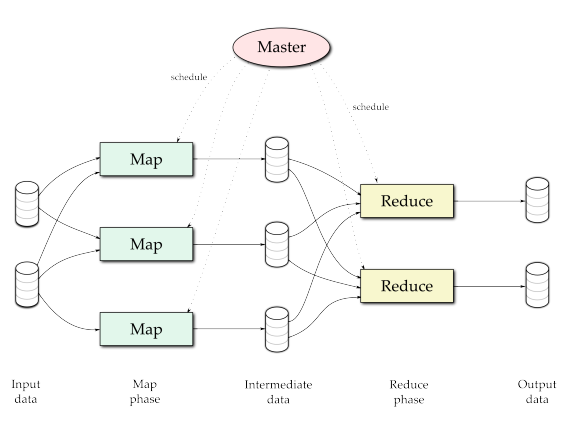
\includegraphics[width=0.8\textwidth]{./images/mapReduceModel.png}
\caption{MapReduce workflow} \label{fig:mapreducemodel}
\end{figure}


Mappers start processing its associated data block and emit key/value pairs. Each mapper output is allocated to a particular reducer by the application's partition function; pairs with the same key are sent to the same reducer. Between the map and reducer stages, the intermediate data is shuffled in order to move it from map nodes to its reduce nodes. This shuffle phase is started as soon as mappers produce pairs. After all mappers Finnish and shuffle phase completes, reducers move into the reduce phase, where the reduce function is applied to the intermediate data and the final output is written.
\par





